\subsection{RQ3: Causal Effect of Validation per Hallucination Class (E2)}
\label{sec:res-inject}
E2 removes model stochasticity: a scripted provider returns an oracle plan derived from S6's real evidence (\texttt{TRIM\_WHITESPACE}, two \texttt{STANDARDIZE\_CATEGORY} mappings, \texttt{STANDARDIZE\_DATE\_FORMAT}, \texttt{FILL\_MISSING(median)}) and one injected hallucination. Hallucinations either \emph{append} an extra recommendation (+) or \emph{substitute} for their correct counterpart ($\leftrightarrow$), as a real model would. Table~\ref{tab:inject} and Fig.~\ref{fig:inject} report the outcomes.

\begin{table*}[t]
\centering
\caption{E2 hallucination injection on S6 (13 corruptions; deterministic, so no variance). \emph{Mode}: + appended to the oracle plan, $\leftrightarrow$ substituted for its correct counterpart. \emph{Verdict}: the validator's decision on the injected recommendation and the first failing rule. \emph{Dmg}: originally clean cells modified plus original rows lost. ``Run aborted'': executor fail-fast stop, no output written.}
\label{tab:inject}
\footnotesize
\begin{tabular}{@{}llclcccc@{}}
\toprule
& & & & \multicolumn{2}{c}{\textsc{AI\_Only}} & \multicolumn{2}{c}{\textsc{Converge}}\\
\cmidrule(lr){5-6}\cmidrule(lr){7-8}
\textbf{ID} & \textbf{Hallucination class} & \textbf{Mode} & \textbf{Verdict} & \textbf{Recall} & \textbf{Dmg} & \textbf{Recall} & \textbf{Dmg}\\
\midrule
\tabinput{../tables/injection.tex}
\bottomrule
\end{tabular}
\end{table*}

\begin{figure}[t]
\centering
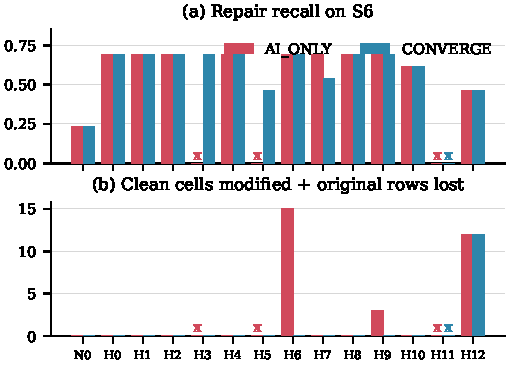
\includegraphics[width=\columnwidth]{injection.pdf}
\caption{E2 per-case outcomes on S6. An ``x'' marks an aborted run (no output).}
\label{fig:inject}
\end{figure}

The thirteen cases fall into five groups.

\noindent\textbf{(i) Caught by structure alone (H1, H2).} Invented and forbidden operation names are dropped by \textsc{AI\_Only}'s structural filter as well; both arms yield the oracle result. A closed operation catalog is, by itself, an effective first line of defence---an argument for recommendation over code generation.

\noindent\textbf{(ii) Availability failures prevented (H3, H5).} A phantom column or an out-of-domain parameter is caught by the executor's defence-in-depth checks under \textsc{AI\_Only}, but fail-fast semantics then \emph{abort the entire run}: one hallucinated recommendation discards every correct repair. \textsc{Converge} rejects the bad recommendation up front and executes the rest (H3: recall $0.69$; H5: $0.46$, since the substituted date operation is lost).

\noindent\textbf{(iii) Silent corruption prevented (H6, H9).} These are the most dangerous cases, because \textsc{AI\_Only} \emph{succeeds}. H6 smuggles an extra \texttt{sql} key into an otherwise valid \texttt{NORMALIZE\_CASE} on \texttt{city}; the executor ignores unknown keys, upper-cases the column, and damages 15 clean cells. H9 proposes \texttt{REMOVE\_DUPLICATES} on criteria \{\texttt{department}, \texttt{city}\}, which no evidence supports; \textsc{AI\_Only} silently deletes three \emph{original} employee records. \textsc{Converge} rejects both (unexpected parameter; no exact-criteria duplicate evidence) with zero damage.

\noindent\textbf{(iv) Conservativeness costs (H7, H8, H4).} H7 adds one fabricated key (\texttt{Engg.}) to an otherwise correct mapping. The fabricated key is harmless at execution time, so \textsc{AI\_Only} keeps all repairs (recall $0.69$), whereas \textsc{Converge} rejects the whole recommendation and loses two correct category repairs ($0.54$). This is the only case in which unvalidated AI outperforms validated AI. H8 (a contradicted null count) is rejected, leaving two salaries missing instead of incorrectly imputed: equal recall, but $2$ fewer incorrect repairs. H4 (trimming an integer column) is rejected on dtype but would have been a no-op.

\noindent\textbf{(v) Beyond the reach of validation (H10, H11, H12).} H10 maps the \emph{real} variant \texttt{mARKETING} to \texttt{Sales}. Every checkable predicate holds, the validator approves it, and both arms produce the same incorrect repair. H12 reproduces the evidence-type conflation observed in E1: whitespace evidence licenses a lowercase of \texttt{name}, which is approved and damages 12 clean cells in both arms. H11 proposes a constant \texttt{"unknown"} for an integer column; the parameter is a well-typed string, so the validator admits it at the \textsc{review} tier, and the executor's coercion check then aborts the run in \emph{both} arms. H11 identifies a concrete gap---type-coercibility of constant fill values is checkable from the profile and should be validated---whereas H10 is the irreducible class discussed in \S\ref{sec:discussion}.

\noindent\textbf{Summary.} Of the eleven checkable classes (H1--H9, H11, H12), the validator rejected nine. It turned two run aborts into successful partial cleaning and prevented 15 corrupted cells and 3 lost records. It cost two correct repairs in one case. The no-op control N0 (recall $0.23$) confirms that three whitespace repairs are performed by Spark's CSV writer irrespective of the plan.
